\documentclass[a4paper,10pt]{book}
\usepackage[ngerman]{babel}							%Sprache
\usepackage[utf-8]{inputenc}						%Umlaute ohne Maske
\usepackage{amsmath}								%Mathe fr alle!
\usepackage{amsfonts}								%Mathefonts
\usepackage{graphicx}								%Bessere Grafikunterstzung
\usepackage[pdfborder = 0 0 0]{hyperref}			%Nette PDFs ohne Mh...
\usepackage{fancybox}
\usepackage{listings}

\title{PPLT2 Handbuch}
\author{Hannes Matuschek \texttt{<hmatuschek@gmx.net>}}


\newenvironment{merke}%
    {\begin{center}\bfseries\begin{Sbox}\begin{minipage}{10cm}\parskip=2ex}%
    {\end{minipage}\end{Sbox}\fbox{\TheSbox}\end{center}}


\begin{document}
	\parindent = 0em
	\parskip = 2ex


\chapter{Theorie}
\section{Ziele}
    Ziel der PPLT2 ist ein Framework für Master-Slave basierte Kommunikation. 
    Dabei sollen die einzelnen Komponenten des Kommunikationsweges, das sind 
    Schnittstellen zur Hardware, Transportprotokolle, 
    Kommandonachtrichtenformate und die Verarbeitung von Werten in einzelnen 
    Modulen implementiert werden. Das bedeutet aber auch, dass das Framework 
    von sich aus keinerlei Fähigkeiten zur Kommunikation besitzt. 
    Die seperate Implementation der einzelnen Kommunikationsschichten stellt
    sicher, dass Module häufig wieder verwendet werden können, was die 
    Programmierarbeit, die benötigt wird um ein neues Gerät ansprechen zu 
    können, minimiert. 
    
    Daraus ergibt sich die Forderung nach einer klaren Definition der 
    Intermodul-Schnittstellen\footnote{\emph{Intermodul} bezeichnet die 
    Schnittstellen, die Module anbieten müssen, damit andere Module darauf 
    zugreifen können. Auf der anderen Seite kann der Entwickler erwarten, 
    das die durch die Schnittstellendefinition erforderten Methoden auch
    wirklich vorhanden sind.}, da zur Zeit der Implementation des Moduls 
    nicht bekannt seien kann, in welchem Kontext das Modul verwendet wird.
    
    Eben dies wird von der PPLT zur Verfügung gestellt. 
    \begin{itemize}
    \item Eine klare syntaktische Definition der Intermodul-Schnittstellen. 
        Syntaktisch bedeutet in diesem Fall, dass genau definiert ist, welche
        Methoden durch eine Modul-Klasse implementiert werden müssen, um der 
        Schnittstellendefinition zu entsprechen. Praktisch wird dies duch eine
        Klasse realisiert, von der die Modul-Klasse abgeitet werden \textbf{muss}.
        Dadurch wird sichergestellt, dass alle benötigten methoden vorhanden 
        sind.
    \item Eine eindeutige semantische Definition der Funktionsweise der
        Modulmethoden. Sematisch bedeutet, dass definiert ist wie sich
        ein Modul zu verhalten hat. Dadurch kann auf eine genaue Kenntnis
        der Funktionsweise von Module verzichtet werden. Da alle Module sich
        gleich verhalten müssen. Da das Verhalten zur Kompilezeit nicht 
        geprüft werden kann, ist die Disziplin des Programmieres gefragt.
        Eine Fehlerhafte Implementation kann zu sehr obskuren Fahlern im
        Programmablauf führen.              
    \item Eine Umgebung zur Verwaltung von Modulen. Die Verwaltung stellt
        Ihnen Werkzeuge zur Verfügung, mit denen sie Module bequem laden,
        entladen und verbinden können.  Dies ist auch zur Laufzeit möglich.
        Somit können Sie zu einem beliebigen Zeitpunkt eine Kommunikation
        zu einem Gerät oder sonstiegen Informationsquellen aufbauen oder 
        schließen.
    \item Es werden außerdem Werkzeuge zur Entwicklung und zum Entwanzen
        eigener Module bereit gestellt. Dies sind meißt Module, die 
        die Verhalten der Eigenentwicklungen überwachen oder mit denen
        sich eine Umgebung emulieren lassen, die einem realen Umfeld 
        entsprechen.
    \end{itemize}
    
    
    \subsection{Anwendungsgebiete}
    Das primäre Anwendungsgebiet der PPLT ist die Ausbildung von Fachkräften.
    Sie soll ein Verständniss des generellen Aufbauis einer Master-Slave 
    Kommunikation mit Geräten vermitteln. An Ihr können Begriffe wie das OSI 
    Refrenzmodell anschaulich dargestellt werden, indem ein einzelnes Modul 
    der PPLT mit einer Schicht im Referenzmodell assoziiert wird. Des weiteren 
    wurde versucht die Intermodulschnittstellen so einfach wie möglich zu 
    halten um eine schnelle und einfache Entwickung eigener Module Rechnung zu 
    tragen. 
   

\section{Master-Slave Kommunikation und deren Abbild auf die PPLT}    
    \subsection{OSI-Referenzmodell}
    \label{sec:th_osilayer}
    Im OSI Referenzmodell wird die Kommunikation in verschiedene Schichten 
    (Layer) aufgespalten. Die niedrigste Schicht genannt die physikalische 
    Schicht definiert und behandelt die physikalische Übertragung der 
    Information. Die oberste Schicht, die Anwendungsschicht, behandelt die
    Verarbeitung der übertragenen Daten, eben die Anwendung. Die Philosophie
    dieses Modells ist, dass sich jede Kommunikation in einzelne Schichten,
    die völlig unabhänging von einander operieren, zerlegen lässt. Diese Idee
    soll auch in der PPLT Anwendung finden. Jede Schicht des OSI 
    Referenzmodells sollte nach Möglichkeit als ein einzelnes Modul 
    implementiert werden. Die Module müssen völlig unabhängig von einander
    funktionieren. Es darf niemals sein, dass ein bestimmtes Modul von
    einen anderen Modul abhängt. In diesem Falle sollten beide Module
    zu einem zusammen gefasst werden.
    
    Daraus leitet sich der erste Schritt im Entwicklungszyklus eines Moduls ab:

    \begin{merke}
        Zu allererst muss das zu behandelne Problem mit dem OSI 
        Referenzmodell verglichen werden. Die einzelnen Schichten müssen 
        identifiziert werden. Dieser Schritt bedarf Sogfalt. Eine 
        Fehlentscheidung an dieser Stelle kann dazu führen, dass die 
        Entwicklung der einzelnen Module sich als sehr schwierig gestaltet 
        im schlimmsten Fall sogar nicht zuverlässig arbteiten.
    \end{merke}

    Es ist wie Eingangs erwähnt auch möglich, dass einzelne Schichten zu einem
    Modul zusammen gefasst werden können oder sogar müssen, wenn diese Schichten
    nicht Unabhänging von einander sind. Es sollte außerdem noch erwähnt sein,
    dass häufig die Anwendungsschicht und die pysikalische Schicht nicht durch 
    Module implementiert werden. Die Anwendungsschicht wird häufig durch 
    Visualisierungen repräsentiert und um die physikalische Schicht kümmert
    sich meist das Betriebssystem. Es bleiben also nur die Schichten 
    dazwischen, die durch Module implementiert werden müssen.
    
    Es wäre nun an der Zeit mal ein einfaches Beispiel zu nennen.
     
    Ein sehr einfaches Beispiel wäre die Kommunikation mit einem 
    Mobiltelefon über dessen serieller Schnittstelle (COM-PORT).
    Über diese Schnittstelle kann man viele Werte des Telefons 
    abfragen oder aber auch SMS senden/emfangen. Das Telefon erwartet vom
    COM-Port eine Zeichenkette, die aus einem Befehl (AT-Kommando) einem
    meißt optionalen Parameter und einem definiertem Zeilenende besteht. 
    Man brauch also nur irrgendwie auf die serielle Schnitstelle einen 
    lesbaren String zu schreiben und die Antwort (wieder eine Textzeile)
    zu interpretieren! 
    
    Der Dialog könnte auf der serielle Schnittstelle so aussehen:
    \begin{lstlisting}
        <<< ATZ\r\n
        >>> OK\r\n
        <<< AT+CBC\r\n
        >>> AT+CBC 90\r\n
        >>> OK\r\n
    \end{lstlisting}
    
    Hier wurde der aktuelle Batteriestand des Telefons abgefragt, wobei 
    \texttt{<<<} senden bedeutet und \texttt{>>>} empfangen. 
        
    Durch dieses einface Protokoll reduziert sich das OSI Modell auf 4 
    Schichten. Davon sind die physikalische Schicht und die Anwendungsschicht 
    schon mal fertig. Um die physikalische Schicht kümmert sich der UART 
    Controller im PC, die Anwendung sei hier mal ganz hypothetisch schon 
    fertig. Es muss also nur noch ein Modul geschrieben werden, welches den 
    Zugriff auf die serielle Schnittstelle ermöglicht (\texttt{COM}) und ein 
    Modul, das die Kommandos des Mobiltelefons erzeugt und verstehen kann 
    (\texttt{HANDY}). Wie dass im einzelnen geschehen muss, wird später noch 
    erklärt. Nun werden die Module übereinander gelegt. Das COM-Modul liegt 
    unten, da es direkt mit dem Betribssystem arbeitet. Das HANDY-Modul liegt 
    darüber und greift somit auf das COM-Modul zu (siehe Abb 
    (\ref{fig:osi_handy_com})).
    % FIXME Assoziation mit den OSI Schichten
    
    
    \begin{figure}
        \centering
        \begin{picture}(150,70)
            \put(5,60){\dashbox{2}(140,20){Anwendung}}
            \put(5,40){\framebox(140,20){HANDY - Modul}}
            \put(5,20){\framebox(140,20){COM - Modul}}
            \put(5,0){\dashbox{2}(140,20){Betribssystem}}
        \end{picture}
        \caption{OSI Modell der PC-Handy-Kommunikation}
        \label{fig:osi_handy_com}
    \end{figure}

    \subsection{Feinstruktur}
    Nachdem die Kommunikation in ihre Einzelteile (Schichten) zerlegt wurde, 
    ist es Zeit zu überlegen, was zwischen den einzelnen Schichten 
    ausgetauscht wird. Dazu schaut man sich den Protokollablauf noch etwas 
    genauer an. Ein geignetes Diagramm wäre das in Abb 
    (\ref{fig:osi_handy_time}). Dort werden die einzelnen Schichten als 
    sekrechte Striche eingezeichnet und benannt. Die 'y-Achse' ist die Zeit. 
    Nun trägt man mit Pfeilen die Interaktionen ein, wobei der Pfeil immer
    vom Aufrufenden zum Aufgerufenen zeigt! Die gestrichelten Pfeile sind 
    die Antworten der aufgerufenen auf eine Frage (Fragen enden wie im
    echten Leben mit einem Fragezeichen). So wird das COM-Modul auf die
    Frage nach Daten mit einem Datensatz antworten es sei den ein Fehler
    (z.B. ein Timeout) tritt auf. Was ist aber nun mit den Pfeilen, die
    keine Fragen oder Antworten sind? Nun, das sind Befehle der Art 
    \textbf{sende}. Man könnte also das Diagramm (\ref{fig:osi_handy_time})
    wie folgt lesen. 
    
    \textit{ Die Applikation \textbf{fragt} das Handy-Modul nach dem
        Batteriestand. Das Handy-Modul \textbf{sendet} darufhin den 
        entsprechenden Befehlsstring an das COM-Modul. Das COM-Modul
        \textbf{sendet} diesen String dann an das Betribssystem also
        an die serielle Schnittstelle. Damit wäre die Transaktion 
        zunächst beendet. Doch nun \textbf{fragt} das Handy-Modul 
        das COM-Modul ob eine Antwort (Daten) vorliegen. Das 
        COM-Modul weis das natürlich noch nicht und \textbf{fragt}
        daraufhin die serielle Schnittstelle. Vorausgesetzt, dass alles in 
        Ordnung ist, wird die serielle Schnittstelle (Betriebsystem)
        Daten empfangen haben und diese an das COM-Modul \textbf{zurückgeben},
        welches diese Daten wieder an das Handy-Modul \textbf{weiter gibt}.
        Das Handy modul analysiert die Antwort und \textbf{gibt} den 
        ermittelten Wert an die Applikation zurück.
    }
    
    Stellt man nun für alle zu implementierende Fälle ein solches Diagramm auf, 
    so stellt man fest, dass sich die Interaktion immer auf ein solches 
    senden-empfangen Scenario reduzieren lässt. Voraussetzung ist jedoch,
    dass man bei der Zerlegung in Schichten die richtigen Entscheidungen 
    getroffen hat. Schon an dieser Stelle kann man eine Schlechte Zerlegung
    erkennen, wenn sich die Kommunikation nicht allein durch lese und schreib
    Zugriffe ausdrücken lassen. 
    
    \begin{figure}
        \centering
        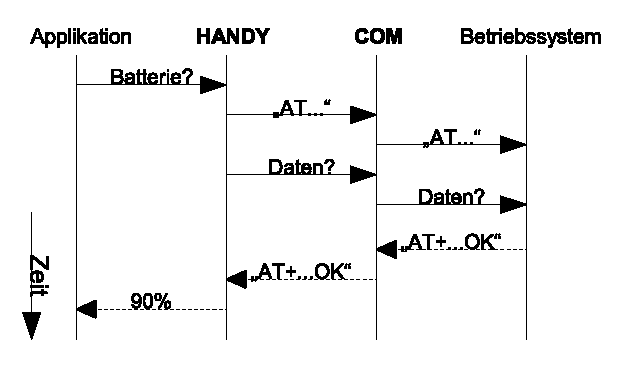
\includegraphics[scale=.8]{osi-handy-time.eps}
        \caption{Zeit verlauf der einzelnen aufrufe...}
        \label{fig:osi_handy_time}
    \end{figure}

    So lässt sich die erste Design Regel der PPLT wie folgt definieren;
    \begin{merke}
        Jedes Modul muss die Methoden \textit{lesen} und \textit{schreiben}
        implementieren. Die genauen Namen dieser Methoden sind bei 
        unterschiedlichen Datentype der ausgetauschenten Information duchraus
        unterschiedlich. Wobei die methode \textit{lesen} einer Frage nach
        Daten und die Methode \textit{schreiben} dem Senden von Daten 
        gleich kommt. Diese Methoden werden immer von dem Modul (oder
        besser: der Schicht) aufgerufen, das oberhalb des eingenen 
        Moduls liegt.
        
        Daraus ergibt sich, dass nur benachbarte Module miteinander 
        interagieren können. Außerdem können sich benachbarte Module immer nur
        die selben Befehle geben oder die selben Fragen stellen! Dies erscheit
        zunächst sehr einschränkend, jedoch wird man nie erwarten, dass das 
        COM-Modul eine Frage nach dem Batteriestand beantwortet.
        Sie mögen mir an dieser Stelle dennoch wiedersprechen, da sie ja 
        wissen, dass man dem Handy-Modul durchaus verschiedene Fragen stellen 
        kann. Zum beispiel nach dem Batteriestand, der aktuellen Signalstärke,
        ... Dieses scheinbare Paradoxum wird jedoch in der Sektion 
        \ref{sec:th_adressen} aufgelöst. 
    \end{merke}

    
    
    \subsection{Addressierung}
    \label{sec:th_adressen}
    In diesem Abschnitt werde ich die Frage beantworten, wie es möglich sein
    soll, dass ein Modul dem anderen immer nur die selbe Frage stellen kann,
    aber das Module \texttt{Handy} durchaus verschiedene Fragen verstehen 
    soll! Die Antwort daruf ist recht einfach: \textit{Jedes Modul kann
    durchaus mehrere Module besitzten, die darauf rumliegen!} Um sich 
    ein Bild davon zu machen, wie man sich soetwas vorstellen soll,
    muss das Diagramm aus dem Abschnitt \ref{sec:th_osilayer} etwas 
    modifiziert werden. In einem solchen Diagramm 
    (Abb (\ref{fig:mod_tree})) liegen die Module nicht einfach aufeinander, 
    sondern sind durch einfache Striche miteinander verbunden.
    
    \begin{figure}
        \centering
        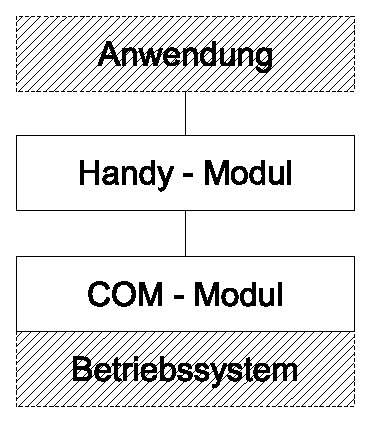
\includegraphics[scale=.8]{mod-tree.eps}
        \caption{Module in der Baumansicht.}
        \label{fig:mod_tree}
    \end{figure}
    
    Diese Konfiguration entspricht dem Beispiel der oberen Abschnitte.
    Nun könnte die Applikation (z.B ein kleines Programm) noch nach der 
    Aktuellen Signalstärke fragen. Diese Frage würde natürlich wieder an das
    Handy-Modul gestellt werden. Damit dieses Modul die Frage \emph{Batterie?}
    und \emph{Signalstärke} unterscheiden kann wobei lediglich der 
    Methodenaufruf \emph{lesen} verwendet werden kann, muss mann dem
    Modul auf irrgend eine Weise bekannt geben wonach gefragt wird. Dies 
    geschieht durch Verbindungen die Adressen besitzen. Eine Abbildung
    dieser Konfiguration ist die Abbildung (\ref{fig:mod_tree2}).
    
    
    \begin{figure}
        \centering
        \includegraphics[scale=.8]{mod-tree2.eps}
        \caption{}
        \label{fig:mod_tree2}
    \end{figure}

    Hier besitzt das Handymodul zwei \textbf{Anschlüsse}, die
    die verschiedenen Werte liefern können. Das COM-Modul bleibt
    unverändert. Um die Anschlüsse zu unterscheiden, werden diesen Adressen
    zugewiesen. In diesem Beispiel bedeutet die Adresse \emph{sig} das beim 
    Lesen die aktuelle Signalstärke und die Adresse \emph{bat} beim Lesen
    der Aktuellen Batteristatus zurückgegeben wird.
    
    Damit sich die Applikation oder aber auch ein anderes Modul mit dem 
    Handymodul verbinden kann, muss dieses eine Methode bieten, die
    \emph{verbinden} heist. Somit ergibt sich eine weitere Forderung an
    \textbf{jedes} Modul.
    
    \begin{merke}
        Jedes Modul muss eine Methode zur Verfügung stellen, mit der sich
        ein anderes Modul oder aber auch die Applikation mit dem Modul
        verbinden kann. Der Rückgabewert dieser Methode muss ein Objekt
        sein, welches die Verbindung zwischen den Modulen repräsentiert.
        Jede Verbindung besitzt eine Adresse! Jede Verbindung ist gerichtet!
        Das bedeutet, das das Modul, welches auf einem Anderen liegt, die
        Verbindung \emph{zum} darunterliegenden besitzt. Die Verbindung geht
        also von Oben nach Unten! 
        
        Die Klasse dieses Verbindungsobjektes wird von der PPLT bereit gestellt.
        Sie müssen sich also nicht weiter um dieses Objekt kümmern. Sie 
        erzeugen einfach eine Instanz dieser Klasse und geben diese zurück, 
        Fertig ist die Laube.
    \end{merke}
    
    Aus dem Diagramm (\ref{fig:mod_tree2}) ist außerdem ersichtlich, dass 
    jedes Modul zwar viele Anschlüsse zur Verfügung stellen kann, jedoch nur
    eine Verbindung zum Modul darunter (wenn überhautp) besitzt. Dadurch 
    ensteht zwangläufig ein so genannter Baum\footnote{Übrigens: Viele Bäume 
    nennt man auch in der Informatik Wald.}. Bäume haben immer \textbf{eine}
    Wurzel aber viele Blätter! In diesem Beispiel ist das COM-Modul die 
    Wurzel, da kein Modul mehr unter der Wurzel liegt! Module  die an das Handy
    Modul ankoppeln wären dann die Blätter. 
    Nun möchte ich an dieser Stelle einige neue Begriffe einführen.
    Als erstes den \emph{Knoten}. Ein Knoten ist hier immer ein Modul!
    Ein Knoten kann höchstens ein Elternelement (Das Modul auf dem der 
    Knoten liegt) haben. Module, die keine Eltern besitzten nennt man
    Wirzel-Elemente (-Knoten). Als Kind-Elemente (-Knoten) bezeichnet
    man die Module, die auf dem Knoten liegen. 
    
    So ist das COM Module ein Wurzelknoten, das Handy Modul ist 
    Kindknoten vom COM Modul und hat dieses als Elternelement.
    Ich werde im folgenden immer von Eltern und Kindern reden.
    
    Ich fasse mal kurz die bisheriegen Theoretischen Ideen der PPLT zusammen:
    \begin{merke}
        Ein Modul implementiert immer \emph{eigenständige} Schicht(en) des OSI
        Referenzmodells.
        
        Ein Modul kann immer nur über die Methoden \emph{lesen} und 
        \emph{schrieben} angesprochen werden. Ist es nicht möglich, das 
        Problem so zu lösen, müssen ggf. Module zusammengefasst werden.
        
        Ein Modul muss die Methode \emph{verbinden} zur Verfügung stellen,
        die aufgerufen wird, wenn sich ein anderes Modul oder die Anwendung
        mit ihm verbinden will. Diese Methode muss ein Verbindungsobjekt 
        zurückgeben, über das das Kindelement mit dem Modul kommuniziert.
        
        Ein Modul kann immer mehrere Kinder Besitzen aber immer höchstens ein
        Elternelement!
        
        Module, die keine Eltern besitzen, heißen Wurzelmodule (engl. 
        Root-Module)
    \end{merke}
    
    Damit wäre das theoretische Fundament weitest gehend abgeschlossen. Es 
    fehlen nur noch die Datentypen die ein Modul liefern kann. Doch dieses
    Kapitel überschneidet sich recht stark mit der Praxis, da dort schon die
    ersten Hacks auftauchen.
    
    \subsection{Datentypen}
    \label{sec:th_datentypen}
    Im vorieren Kapitel haben Sie gesehen, dass ein Modul durchaus 
    verschiedene Informationen durch \emph{Anschlüsse} liefern kann.
    Es ist weiterhin offensichtlich, dass diese nicht immer die selben
    Datentypen besitzen müssen. Außerdem können vierschiedene Module
    auch Daten verschiedener Datentypen erwarten! Dieses Kapitel wird
    Ihnen einen Überblick über die vorhandenen Datentypen geben.
    
    Der Datentyp eines Anschlusses wird über das Verbindungsobjekt
    assoziiert. Das bedeutet, das es eine vielzahl an verschiedenen
    Verbindungsobjekten gibt, für jeden Datentyp eins. Der Typ
    des Anschlusses definiert sich durch die Klasse des Verbindungsobjektes,
    welches bei einem \emph{verbinden} Aufruf zurückgegeben wurde.
    
    Im folgenden will ich eine kleine Übersicht geben, über die von den PPLT
    unterstützten Datentypen. Zu jedem Typ werde ich eine kurze Erklärung und
    ggf. eine typische Anwendung geben.
    
    \subsubsection{Der Datenstrom}
    Der wichtigste Typ ist der Datenstrom. Mit ihm werden Rohdaten,
    wie sie von der Hardware oder einer TCP Verbindung kommen 
    weitergegeben.  
    

\end{document}
